%%%%%%%%%%%%%%%%%%%%%%%%%%%%%%%%%%%%%%%%%%%%%%%%%%%%%%%%%%%%%%%%%%%%%%%%%%%%%%%
%% LaTeX-Vorlage für Abschlussarbeiten                                       %%
%% (TH Köln -Campus Gummersbach, Fak. 10)                                    %%
%%                                                                           %%
%% Gemäß dem Merkblatt zur Anfertigung von Projekt-, Bachelor-, Master- und  %%
%% Diplomarbeiten der Fakultät 10 von Frau Prof. Dr. Halfmann &              %%
%% Herr Prof. Dr. Rühmann (Version vom 27.01.2008)                           %%
%%                                                                           %%                                                                            
%% Bitte sprechen Sie unbedingt mit Ihrer Betreuerin bzw. Ihrem Betreuer     %%
%% bezüglich der Ausgestaltung Ihrer Arbeit!                                 %%
%%                                                                           %%
%%                                                                           %%
%% MERKKASTEN IN DIESER VORLAGE:                                             %%
%% In dieser Vorlage finden Sie Merkkasten, die Ihnen Informationen          %%
%% zu bestimmten, formalen Aspekten geben. Sprechen Sie immer auch mit       %% 
%% Ihrer Betreuerin bzw. Ihrem Betreuer dazu an.                             %%                       
%% Für die eigene Verwendung der Vorlage entfernen oder kommentieren Sie die %%
%% Merkkasten. Die betreffenden Bereiche für die Merkkasten in der Vorlage   %%
%% sind wie folgt kommentiert: <MERKKASTEN> ... </MERKKASTEN>.               %%                            %%                                                                           %%
%%                                                                           %%
%% LIZENZ:                                                                   %%
%% Diese Vorlage darf nicht kommerziell verbreitet                           %%
%% werden. Eine nicht-kommerzielle Weitergabe ist                            %% 
%% gestattet.                                                                %%
%%                                                                           %%
%% Von Ludger Schönfeld, M. Sc.,                                             %%
%% 2014-2017                                                                 %%
%%%%%%%%%%%%%%%%%%%%%%%%%%%%%%%%%%%%%%%%%%%%%%%%%%%%%%%%%%%%%%%%%%%%%%%%%%%%%%%

%%%%%%%%%%%%%%%%%%%%%%%%%%%%%%%%%%%%%%%%%%%%%
%% HEADER                                  %%
%%%%%%%%%%%%%%%%%%%%%%%%%%%%%%%%%%%%%%%%%%%%%
\documentclass[a4paper,12pt,oneside]{article}
% Optionen:
% - a4paper => DIN A4-Format
% - 12pt    => Schriftgröße (weitere  
%              grundlegende Fontgrößen: 10pt, 11pt)
% - oneside => Einseitiger Druck

%% Verwendete Pakete:
\usepackage[ngerman]{babel} % für die deutsche Sprache
\usepackage{caption} % Für schönere Bildunterschriften
\usepackage[T1]{fontenc} % Schriftkodierung (Für Sonderzeichen u.a.)
\usepackage[utf8]{inputenc} % Für die direkte Eingabe von Umlauten im Editor u.a.
\usepackage{fancyhdr} % Für Kopf- und Fußzeilen
\usepackage{lscape} % Für Querformat

%% Schriften (Beispiele)
%% Weitere LaTeX-Schriften im "LaTeX Font Catalogue"
%% unter: http://www.tug.dk/FontCatalogue/.
%% ACHTUNG: Ggf. müssen Schriften noch installiert 
%% werden!

% Serifen-Schriften:
\usepackage{lmodern} % Schriftart "Latin Modern"
%\usepackage{garamond} % Schriftart "Garamond"

%Sans Serif-Schriften:
%\usepackage[scaled]{uarial}
%\usepackage[scaled]{helvet}
%%--------------
\usepackage[normalem]{ulem} % Für das Unterstreichen von Text z.B. mit \uline{}
\usepackage[left=3cm,right=2cm,top=1.5cm,bottom=1cm,
textheight=245mm,textwidth=160mm,includeheadfoot,headsep=1cm,
footskip=1cm,headheight=14.599pt]{geometry} % Einrichtung der Seite 

\usepackage{graphicx} % Zum Laden von Graphiken
% INFO: Graphiken einbinden
%
% \includegraphics[scale=1.00]{dateiname}
%
% => Ausgabeformat: PDF-Dokument:
%    Es können die folgenden (Graphik-)formate eingebunden
%    werden: .jpg, .png, .pdf, .mps
% 
% => Ausgabeformat: DVI/PS:
%    Folgende (Graphik-)formate werden unterstützt:
%    .eps, .ps, .bmp, .pict, .pntg
\usepackage{epstopdf}

% Pakete für Tabellen
\usepackage{tabularx} % Einfache Tabellen
\usepackage{longtable} % Tabellen als Gleitobjekte (für die Aufteilung bei langen 
 %Tabellen über mehrere Seiten)
\usepackage{multirow} % Für das Verbinden von Zeilen innerhalb einer Tabelle mit
 % \multirow{anzahl}{*}{Text}

% (Zusatz-)Pakete für Formeln
\usepackage{amsmath}
\usepackage{amsthm}
\usepackage{amsfonts}

\usepackage{setspace} % Paket zum Setzen des Zeilenabstandes
% INFO: Zeilenabstand setzen:
%
% Befehle:
% - \singlespacing  => 1-zeilig (Standard)
% - \onehalfspacing => 1,5-zeilig
% - \doublespacing  => 2-zeilig 
\onehalfspacing % Zeilenabstand auf 1,5-zeilig setzen

% Farbboxen (für die Merkkästen in dieser Vorlage):
\usepackage{tcolorbox}
\tcbset{colback=white,colframe=orange,
        fonttitle=\bfseries}

\usepackage[colorlinks,pdfpagelabels,pdfstartview=FitH,
bookmarksopen=true,bookmarksnumbered=true,linkcolor=black,
plainpages=false,hypertexnames=false,citecolor=black]{hyperref} % Für Verlinkungen
% INFO: Verlinkungen mit dem hyperref-Paket:
%
% Die Angabe von URLs mit dem Befehl \url{} erlaubt einen
% gesonderten Umgang mit Weblinks. Denn die Links werden verlinkt.
% Auch erfolgt automatisch am Zeilenende ein Umbruch des Links.
% Es ist auch nicht erforderlich, Sonderzeichen in der URL manuell zu 
% entschärfen.
%
% TIPP: Sollte ein Umbuch bei einem Link nicht automatisch erfolgen, so kann
% das daran liegen, dass ein/mehrere Zeichen zusätzlich angegeben werden müssen,
% an dem der Link umbrochen werden kann.
% Dies kann mit folgendem Befehl erfolgen (Beispiel):
% \renewcommand*\UrlBreaks{\do-\do_}

% Das Paket "biblatex" für autom. 
% Literaturverzeichnisse:
\usepackage{csquotes} % Für sprachangepasste Anführungszeichen
\usepackage[backend=biber,style=authoryear,citestyle=apa]{biblatex}
\addbibresource{bib/literatur.bib}

\title{Entwicklung von Darstellungs- und Interaktionsmöglichkeiten in Virtual Reality für das Cranach Digital Archive}
\author{Nikolas Beckel (11103435)}
\date{15. September 2020}
% Use \maketitle for generated title

%%%%%%%%%%%%%%%%%%%%%%%%%%%%%%%%%%%%%%%%%%%%%
%% DOKUMENT                                %%
%%%%%%%%%%%%%%%%%%%%%%%%%%%%%%%%%%%%%%%%%%%%%
\begin{document}
  \tableofcontents
  \newpage
  \section{Einleitung}
    % \begin{itemize}
    %   \item Das Thema vorzustellen
    %   \item Das Ziel vorzustellen
    %   \item Den Leser neugierig machen
    %   \item Die Relevanz zu beschreiben
    % \end{itemize}
      
    Virtual Reality ist nicht mehr nur Zukunftsmusik oder ein Anwendungsbereich für Forscher
    großer Konzerne. Immer mehr rückt Virtual Reality in den Massenmarkt. Wo zu Beginn
    leistungsfähige Computer benötigt wurden, entstehen nun All-in-One VR-Brillen\footnote{Oculus Quest 2 - All-in-One VR-Brille | \url{https://www.oculus.com/quest-2/} (21.09.2020)}.
    Die Anwendungsbereiche von Virtual Reality sind vielfältig: Gaming, Unterhaltung durch VR-Filme oder
    das Treffen von Freunden in virtuellen Welten\footnote{Mozilla Hubs | \url{https://labs.mozilla.org/projects/hubs/} (21.09.2020)}.
    Die Pandemie durch das Virus SARS-CoV-2 hat uns auch gezeigt, dass immer mehr digitale Lösungen
    benötigt werden. Durch solche Krisen bekommen plötzlich Anwendungsbereiche, die nicht als
    notwendig betrachtet worden, völlig neue Relevanz.
    Durch Virtual Reality ist man nicht mehr an einen Ort gebunden und kann gewisse Aktionen
    statt in der realen Welt, in einer virtuellen Welt ausführen. Da man von der realen Welt
    losgelöst ist, entstehen auch völlig neue Möglichkeiten, diese aufzuführen.
    In dieser Bachelorarbeit wird das digitale Archiv der Cranachs\footnote{Cranach Digital Archive | \url{http://lucascranach.org/} (21.09.2020)}
    als Ressource genutzt, um neue Möglichkeiten der Darstellung für Kunst und Kultur zu erforschen.
    Dabei sollen aktuelle Entwicklungen, unter anderem aus dem musealen Bereich, miteinbezogen 
    und deren Erkenntnisse berücksichtigt werden.
    Auf Basis der recherchierten Ergebnisse sollen ein oder mehrere Prototypen entwickelt werden,
    die zeigen, wie man Virtual Reality im Bereich Kunst und Kultur anwenden kann. Dabei sollen die
    aktuellsten Technologien miteinbezogen und abgewägt werden, mit welcher Technologie die
    besten Ergebnisse erzielt werden können.

  \section{Grundlage und Datenbasis}
    In diesem Kapitel werden auf die Grundlagen von Virtual Reality, auf Lucas Cranach 
    der Ältere und auf das Cranach Digital Archive eingegangen. Letzteres stellt 
    die Datenbasis für dieses Projekt dar, welche in der Entwicklung der Prototypen 
    eingesetzt wird. Dieses Grundwissen wird für das nächste Kapitel benötigt, welches 
    sich tiefgründiger mit Virtual Reality und der Kunstwerke von Lucas Cranach
    beschäftigt.

    \subsection{Das Cranach Digital Archive}
      Das Cranach Digital Archive ist eine Initative und ein visionäres Forschungsprojekt, 
      welches sich zum Ziel gesetzt hat, alle relevanten Informationen, Dokumente und 
      Werke der Cranachs in einer digitalen Datenbank der Forschung und Öffentlichkeit zur 
      Verfügung zu stellen.
      So konnten bisher über 1600 Gemälde und 14000 Abbildungen digitalisiert und auf der 
      Webseite \url{lucascranach.org} veröffentlich werden, welche frei über das
      Internet zugänglich ist.
      Bei den digitaliserten Aufnahmen der Werke handelt es sich nicht nur um hochauflösende
      Gemälde, sondern auch Röntgenaufnahmen, Infrarotreflektogramme und
      Archivalien. Dadurch lassen sich verschiedene
      Gemälde der Cranachs aus einer völlig neuen Perspektive betrachten, denn durch die
      Infrarotreflektogramme lassen sich zum Beispiel Unterzeichnungen
      eines Gemäldes erkennen, welches das bloße Auge niemals sehen könnte. [\cite{heydenreich2017lucas}]
    \subsubsection{Lucas Cranach der Ältere}
      Lucas Cranach d. Ä. war nicht nur ein erfolgreicher Künstler während der Renaissance,
      sondern auch ein guter Freund Martin Luthers und ermöglichten gemeinsam eine moderne 
      Auffassung der Kunst.
      Lucas Cranach d. Ä. wurde 1472 als Sohn eines Malers namens Hans Moller geboren
      und wurde auch von ihm in der Zeichenkunst unterrichtet.
      Obwohl er früh mit dem Malen begonnen hat, wird Lucas Cranach d. Ä. erst in Wien
      um 1502 als Künstler greifbar. Um 1504/05 rum 
      verlässt er Wien und nimmt den Beruf des Hofmalers in Wittenberg für Friedrichs III. 
      entgegen, von dem er auch sein zukünftig verwendetes Wappen verliehen bekommen 
      hat.
      Dieses Wappen, eine \glqq geflügelte, bekrönte und einen Ring im Maul tragende
      Schlange\grqq{} [\cite[15]{heydenreich2017lucas}], sollte fortan als Signet von
      Lucas Cranach und seiner Werkstatt werden.
      Nach dem Tod von Friedrich III., diente er seinem Sohn und Nachfolger
      Johann I., welcher das Amt jedoch nur sieben Jahre lang führen konnte und
      schließlich an seinen Sohn, Johann Friedrich I. abgegeben hat.
      Bis zu Lucas Cranach d. Ä. Tods stand er im Dienst dieser drei Kurfürsten.
      Lucas Cranach d. Ä. zeichnete sind nicht nur in seiner Qualität der Gemälde aus,
      sondern war auch dafür bekannt produktiv zu arbeiten.
      Im Gegensatz zu seiner Konkurrenz malte er nicht einfach nur seine Gemälde an einem
      einfach Ort, sondern baute sich bereits in Wittenberg eine Werkstatt auf, die es
      ihm erlaubte, seine Produktivität auf eine neue Ebene zu bringen.
      Auch die Kunstgattung Druckgrafik, die Martin Luther als Graben bezeichnete, erlaubte
      Lucas Cranach d. Ä. einzelne Gemälde mehrfach zu drucken.
      Er war aber nicht nur als Künstler erfolgreich, sondern belegte in Wittenburg
      zwischen 1519 und 1544/45 das Amt des Ratsherren, einige Jahre davon auch als
      Kämmerer oder Bürgmeister.
      Die letzten Jahre Lucas Cranach d. Ä. waren durch den Schmalkaldischen Krieg
      geprägt und beeinflusst, da Johann Friedrich I. mit seinen Truppen gegen den
      Kaiser kämpfte. Nach einer Niederlage und
      Verlusten seines Territoriums, foltge Lucas Ranach d. Ä. Johann Friedrich I.
      in die Gefangenschaft und verblieb dort von 1547 - 1552.
      Nach der Gefangenschaft kehrte Lucas Cranach d. Ä. nach Weimar zurück und starb
      am 16. Oktober 1553 im Haus seiner Tochter.
      Zusammenfassend war Lucas Cranach d. Ä. nicht nur ein einfacher Künstler, sondern
      war aufgrund seiner Qualität, Produktivität und humanistischem Denken,
      welches sich vor allem in den Gemälden seiner Wiener Zeit wiederspiegelt,
      seiner Zeit voraus und legte einen wichtigen Grundstein für die moderne
      Kunst. [\cite{heydenreich2017lucas}]
    \subsubsection{Martin Luther als Junker Jörg}
      Als Martin Luther 1511 nach Wittenburg zurückkehrte und 1512 die Professur für
      Bibelauslegung übernommen hatte, traf er zum ersten mal auf Lucas Cranach d. Ä.
      Die beiden pflegten nicht nur engen Kontakt zueinander, sondern ergänzten sich auch
      in ihrer Arbeit. Martin Luthsers Gedanken der Reformation konnten nicht nur in
      Schrift verbreitet werden, sondern auch durch Lucas Cranach d. Ä. künstlerischem
      Talent und Produktivität. Martin Luther nahm sogar nachweislich die Dienste von 
      Lucas Cranach d. Ä. für Tiefenholzschnitte entgegen, welche sogar für
      theologische Argumentationen benutzt wurden. Lucas Cranach d. Ä. trug aber auch
      dazu bei, dass es ein öffentliches Bild von Martin Luther gab und versuchte dieses
      auch zu manifestieren. Als 1521 die Reichsacht über Martin Luther verhängt wurde, 
      musste er aus Schutz seinen Tod durch einen inszenierten Überfall vortäuschen.
      Sein enger und guter Freund Lucas Cranach d. Ä. war jedoch über die Inszenierung 
      informiert. 
      Als Martin Luther zurück nach Wittenburg kehrte, um die dortigen Unruhen zu besänftigen, 
      trat er unter dem Pseudonym \glqq Junker Jörg\grqq{} auf. 
      Auch hier nahm Lucas Cranach d. Ä. eine entscheidende Rolle ein, da er auch in dieser 
      Zeit Bildnisse von Martin Luther anfertigte. 
      Beispielsweise wurde zu dieser Zeit ein Bildnisholzschnitt
      von Martin Luther als Junker Jörg gefertigt, welche absichtlich zur Medienstrategie
      verwendet wurde. So überbrachte Lucas Cranach d. Ä. die Nachricht, dass Martin Luther
      den inszenierten Überfall überlebte und vermittelte damit auch das Bild eines 
      entschlossenen und visionären Mannes. [\cite{heydenreich2017lucas}]
      \newline
      In diesem Forschungsprojekt wird sich auf die Datenbasis von Martin Luther als
      Junker Jörg des Cranach Digital Archive bezogen. Zur Entwicklung einer Antwort auf
      die Forschungsfrage wird nicht die gesamte Datenbasis des Cranach Digital Archive
      benötigt, da eine geringe Datenmenge zur Entwicklung von Virtual Reality-Szenen
      bereits ausreichen. Das Team hinter \url{lucascranach.org} hat die Daten bereits
      digitalisiert und aufgearbeitet, weswegen Werke und Gemälde, die miteinander
      verwandt oder in Beziehung stehen, bereits miteinander verknüpft sind.
    \subsection{Konzept und Nutzung von Virtual Reality} \label{Konzept und Nutzung von VR}
      Virtual Reality stammt aus dem Wissenschaftsgebiet der Computergrafik, denn eine
      virtuelle Realität besteht immer aus einer dreidimensionalen Simulation [\cite[13]{Dorner2013}].
      Es gibt mehrere Wege, eine virtuelle Realität zu simulieren. Nicht immer ist eine 
      VR-Brille notwendig, doch ist heutzutage das Nutzen solch einer Brille, um in eine 
      virtuelle Realität einzutauchen, state of the art. Das zeigt auch die schnelle 
      Entwicklung dieser Branche, die vermehrt auf VR-Brillen setzen, welche ohne einen
      zusätzlichen Computer auskommen. Die gesamte Echtzeitsimulation der virtuellen
      Realität wird innerhalb der VR-Brille berechnet\footnote{Oculus Quest 2 - All-in-One VR-Brille | \url{https://www.oculus.com/quest-2/} (21.09.2020)}.
      Sollte die Leistung der Brille nicht ausreichen, lassen sich diese optional mit einem
      Computer verbinden. Bei VR-Displays werden stereoskopische Verfahren angewandt [\cite[13]{Dorner2013}],
      wodurch Objekte, die man durch die VR-Brille sieht, einen Tiefeneffekt erhalten.
      Dieser Tiefeneffekt lässt virtuelle Objekte real erscheinen, da sie erstmals für unser
      Gehirn eine erkennbare räumliche Position aufweisen. Ein weiterer wichtiger
      Bestandteil von Virtual Reality ist die blickabhängige Bildgenerierung [\cite[13]{Dorner2013}].
      Bei der Bewegung des Kopfes, und damit der Blickpunkt des menschlichen Auges, wird
      die virtuelle Welt neu generiert und zwar aus dem Blickwinkel, in welches das
      menschliche Auge in der virtuellen Welt schaut. Da Virtual Reality es erlaubt Objekte
      aus verschiedenen Perspektiven zu sehen und auch mit diesen zu interagieren, gibt
      es vielfältige Einsatzmöglichkeiten. Das Virus SARS-CoV-2 hat gezeigt, dass es
      immer wichtiger wird von zu Hause aus arbeiten zu können oder Dienstleistungen von
      zu Hause aus entgegenzunehmen. Gerade Museen oder Kunstgalerien können von
      Virtual Reality profitieren, da man auf diesem Weg die Kunst auf verschiedene
      Wege übermitteln kann. Man ist nicht mehr an das klassische Bild eines großen
      Raumes mit Gemälden an der Wand gebunden, sondern kann räumliche Limitierungen der
      realen Welt überwinden. Das Cranach Digital Archive ist eine große Datenbank mit
      vielen Gemälden und Archivalien. Einige Gemälde haben eine Beziehung zu anderen 
      Gemälden, da sie zum Beispiel zur selben Zeit entstanden sind oder auf dem selben
      Bildträger angebracht wurden. Virtual Reality kann Forschern, aber auch 
      Kulturinteressierte, dabei helfen, die großen Datenmengen besser aufzunehmen und
      zu verstehen [\cite[9]{Dorner2013}]. Im nächsten Kapitel wird der aktuelle
      Forschungsstand von Virtual Reality erläutert und wie es aktuell für Museen
      eingesetzt wird.

      
      % Grundlagen von VR (Was ist VR überhaupt) und warum ist es im Kontext dieser BA wichtig? 
      % - Darstellung der Kunstwerke in 3D
  \section{Theoretische Einordnung}
    In diesem Kapitel wird sich genauer mit dem Thema Virtual Reality beschäftigt, was 
    der aktuelle Forschungsstand dieser Branche ist und welche Lösungen es bereits auf 
    dem Markt gibt. Mit Hilfe von Fachliteratur zu diesem Themenbereich sollen die
    aufgeworfenen Forschungsfragen beantwortet werden können. Dieses Kapitel stellt das
    wissenschaftliche Fundament für die Entwicklung der Prototypen, die anhand der in
    diesem Kapitel gewonnenen Fakten entwickelt werden sollen. Zunächst wird der aktuelle
    Forschungsstand der VR-Branche betrachtet, welche technologischen
    Möglichkeiten und welche Produkte im musealen Bereich bereits existieren.
    Durch andere VR-Produkte, die ebenfalls im musealen Bereich entwickelt wurden, lassen
    sich Fehler vermeiden und etablierte Ideen für das eigene Produkt umsetzen.
    \subsection{Aktueller Forschungsstand von Virtual Reality}
      Die Idee Kunst in einer virtuellen Realität darzustellen ist keine einzigartige Idee.
      Bereits andere Museen wagten sich daran und stellten Konzepte her, sammelten
      Erfahrungsberichte und entwickelten eigene Produkte\footcite{Heidsiek2019}. Es ist
      aber auch ein richtiger und verständlicher Schritt, dass Virtual Reality immer mehr
      im musealen Bereich Anwendung findet. Denn Museen versuchen Gefühle,
      Erfahrungen und Emotionen zu übermitteln und durch den Einsatz von Virtual Reality
      besteht die Möglichkeit den Besucher in Szenarien zu versetzen, die in der
      Vergangenheit geschehen sind. Der Besucher kann auch Fantasiewelten der Künstler
      wahrnehmen, um ein besseres Verständnis für ihre Kunst zu erlangen. Umfragen ergaben, 
      dass ein Interesse an neuartigen Technologien im Museum vorhanden ist [\cite[34]{Heidsiek2019}].
      Die Besucher erhoffen sich dadurch, dass die Museen unterhaltsamer, lehrreicher und
      zugänglicher werden [\cite[34]{Heidsiek2019}]. Gerade Virtual Reality lässt Museen
      und Informationen zugänglicher werden, denn die Besucher sind nicht mehr gezwungen 
      das Museum physisch zu besuchen. Der Anwendungsbereich ist vielfältig und die 
      Technologie zwar nicht neu, jedoch noch nicht ausgereizt. 
      \subsubsection{Entstehung}
        Virtual Reality ist genau genommen keine neuartige Technologie, sondern existiert
        bereits seit den 60er Jahren. Ivan Sutherland forschte als erster an immersiven 
        Technologien und führte so mit seinem Buch \glqq The Ultimate Display\grqq{} 
        den Rechner, das Design, die Konstruktion und Navigation virtueller Welten zusammen.
        In den 80er Jahren entwickelte NASA erstmals mit dem Projekt VIEW (Virtual 
        Environment Interface Workstations) einen multisensorischen Arbeitsplatz welche für 
        die Simulation virtueller Weltraumstationen genutzt wurde.
        Der Begriff Virtual Reality wurde erstmals 1987 von einem Wissenschaftler namens Jaron
        Lanier verwendet. Er und Thomas Zimmermann gründeten gemeinsam die Firma VPL, welche
        am \glqq DataGlove\grqq{} arbeitete und verkaufte. Der Handschuh konnte mit Hilfe
        von Glasfasern Fingerdaten erfassen. Neben dem Handschuh verkauften sie auch das 
        \glqq EyePhone\grqq{}, eine Weiterentwicklung des Head-Mounted-Displays von Ivan
        Sutherland aus den 60ern.
        1989 wurde ein weiterer Meilenstein erreicht, denn die Firma Polhemus entwickelte 
        einen elektromagnetischen Tracker, welcher ein Ziel in bestimmter Entfernung vom 
        Rechner bestimmen konnte. 
        Zeitgleich entstand BOOM (Binocular Omni-Orientation Monitor) von Fake Space Labs.
        BOOM war ein 3D-Sichtgerät mit einem 1280x1024 Pixel Display, welches 1991 zum 
        ersten Mal Anwendung im \glqq Virtual Windtunnel\grqq{} von Steve Bryson fand, 
        ein Bereich der Luft- und Raumfahrt.
        1988 kamen mehr und verschieden hochwertige Arbeitsplätze für Grafik auf den Markt.
        Silicon Graphics konnte sich mit ihrer SGI Reality Engine 1995 weltweit durchsetzen
        und wurde so zum Standard dieser Branche. Damit kamen dann die ersten kommerziellen
        VR-Softwaresysteme auf den Markt.
        Die nächste große technologische Innovation kam vom Unternehmen SensAble
        Technologies Inc. auf den Markt, welches vom Massachusetts Institut of Technologies
        gegründet wurde. SensAble entwickelte ein haptisches Gerät namens 
        \glqq PHANtom\grqq{} welches man berühren und daraufhin eine
        Kraftrückkopplung spüren konnte.
        Anfang der 90er Jahre, nachdem schon einige technische Innovationen auf dem Markt
        erschienen sind, wurden viele wichtige Forschungen im Bereich der Virtual Reality
        unternommen, welche sich aber auch vor allem auf Stereoleinwände konzentriert haben.
        Nach den Tracking-Systemen auf Basis von Elektromagnetismus folgten Systeme auf
        Basis von von Ultraschall. Gegen 2000 wurde auch der Ultraschall von Infrarot
        abgelöst. Tracking-Systeme auf Basis von Infrafrot finden noch heute Anwendung im
        Bereich der modernen VR-Brillen.
        Die von Silicon Graphics entwickelte SGI Reality Engine, welche in vielen
        VR-Softwaresystemen verwendet wurde, wurde langfristig auch von Computern
        abgelöst, was umfangreichere Forschungen erlaubte, da der Preis um ein fünftel
        gesenkt werden konnte.
        Historisch betrachtet hat auch Deutschland einige Unternehmen vorzuweisen, die sich
        bereits seit 1998 mit VR-Systemen beschäftigen. VRCOM, RTT und IC:IDO sind nur ein
        paar davon.
        Ein ständiger Austausch zum Wissenschaftsgebiet Virtual Reality fand international
        und auf Länderebene statt. Schließlich konnte sich die IEEE VR Konferenz
        international durchsetzen und ist jährlich mit etwa 500 Teilnehmern einer der
        größten Konferenzen zu diesem Thema.
        Seit 2003 hat sogar die Gesellschaft für Informatik eine Fachgruppe für das Thema
        Virtual und Augmented Reality. [\cite[19-21]{Dorner2013}]
        --- --- (Bisschen noch was zum aktuellen Stand schreiben)
      \subsubsection{Wahrnehmungsaspekte} \label{Wahrnehmungsaspekte}
        Wie Menschen Informationen wahrnehmen, ist ein wichtiger Aspekt für die Gestaltung
        von virtuellen Welten. In einer perfekten virtuellen Realität würde der Konsument
        alle Sinneseindrücke die er aus der realen Welt kennt, in der simulierten Welt
        in gleicher Qualität und Quantität empfinden können [\cite[17]{Dorner2013}].
        Doch so eine perfekte virtuelle Realität zu entwickeln ist nach aktuellem Stand
        der Technologie nicht möglich. Die heutigen VR-Systeme und -Technologien
        konzentrieren und beziehen sich auf den visuellen, akustischen und haptischen Sinn
        des Menschens [\cite[34]{Dorner2013}]. Dementsprechend nutzt ein ideales
        VR-System visuelle, akustische und haptische Effekte in Kombination mit einem
        Tracking-System [\cite{Slater2009}]. Die heutige Technologie ist bereits auf
        dem Stand, dass alle drei genannten Sinne angesprochen und beeinflusst
        werden können. Die VR-Brillen selbst besitzen ein Tracking-System für das
        Bewegen des Kopfes, Veränderung der räumlichen Position und 3D-Eingabegeräte,
        die das Bewegen der Hände analysieren können. Die Immersion einer VR-Erfahrung
        wird auch nicht zwingend durch die Bildschirme und das Tracking-System bestimmt,
        sondern an die Anzahl der ausführbaren Aktionen innerhalb der virtuellen 
        Welt [\cite{Slater2009}]. Der technologische Fortschritt der heutigen VR-Brillen
        hilft sehr bei der Entwicklung von virtuellen Welten, jedoch müssen auch die
        durchführbaren Aktionen gut umgesetzt sein. Denn eins der wichtigsten Aspekte
        für das Wahrnehmen von virtuellen Welten ist das Gefühl der 
        Präsenz [\cite{Slater2009}]. Die Präsenz beschreibt das Gefühl, dort zu sein
        [\cite{Slater2009}]. Dabei weiß der Benutzer jedoch zu jedem Zeitpunkt, dass er
        nicht wirklich dort ist [\cite{Slater2009}]. Der Aspekt Präsenz lässt sich in
        drei Unteraspekte aufteilen: Das Gefühl der Ortsillusion, Plausibilitätsillusion
        und Involviertheit [\cite[18-19]{Dorner2013}]. Eine virtuelle Welt sollte immer unter
        Berücksichtigung dieser drei Gefühle entwickelt werden, da eine gute Umsetzung
        dieser die beste Nutzungserfahrung für einen Benutzer sicherstellt. Bei der 
        Ortsillusion handelt es sich um die starke Illusion an einem Ort zu sein, mit dem
        Wissen, dass man nicht wirklich dort ist [\cite{Slater2009}]. Einer der wichtigsten
        Kriterien, um diese Illusion beim Benutzer zu erreichen, ist die zuvor erwähnte
        blickpunktabhängige Bildgenerierung der VR-Brille (siehe Kapitel 
        \ref{Konzept und Nutzung von VR}) [\cite[18]{Dorner2013}]. 
        Bei der Plausibilitätsillusion handelt
        es sich um das Gefühl, dass die Geschehnisse innerhalb der virtuellen Welt 
        wirklich passieren, mit dem Wissen, dass dies nicht wirklich passiert
        [\cite{Slater2009}]. Eine Schlüsselkomponente, um diese Illusion hervorzurufen,
        sind Geschehnisse, die nicht vom Benutzer ausgelöst wurden, sich jedoch auf ihn
        beziehen [\cite{Slater2009}]. Das können beispielsweise auf den Benutzer zufliegende
        Projektile sein oder ein virtueller Mensch, der den Benutzer anspricht
        [\cite[18-19]{Dorner2013}]. Die Geschehnisse die innerhalb der virtuellen Realität
        stattfinden müssen jedoch nicht physikalisch realistisch sein [\cite{Slater2009}], 
        können dementsprechend auch fantasievoll und unrealistisch sein. Als Beispiel kann
        ein Spiel genommen werden, in welchem der Benutzer von einem Magier mit einem 
        Feuerball angeschossen wird. Der Benutzer hat das Ereignis nicht selbst ausgelöst,
        wird jedoch in das Geschehen eingebunden. Eine Plausibilitätsillusion entsteht,
        obwohl das Szenario unrealistisch ist. Die Plausibilitätsillusion kann durch das
        Einbauen von realistischen Effekten, wie Schatten oder die Darstellung des eigenen
        Körpers, verstärkt werden [\cite{Slater2009}]. Das Anzeigen des Körpers des Benutzers
        kann sogar den Effekt der Orts- und Plausibilitätsillusion verstärken, da das
        Gefühl dort zu sein realer erscheint, dementsprechend auch Geschehnisse die den
        Benutzer betreffen [\cite{Slater2009}]. Genauso können beide Illusionen durch das
        Ausnutzen der Ängste eines Menschen hervorgerufen werden [\cite{Slater2009}].
        Leidet der Benutzer unter Höhenangst, dann wird er ebenfalls in der virtuellen
        Welt unter Höhenangst leiden, wenn er sich auf einem Hochaus befindet und die
        Kante herunterschaut. Dementsprechend verstärkt sich das Gefühl, als würde der
        Benutzer sich dort befinden und das aktuelle Geschehnisse gerade passieren. Jedoch
        immer mit dem Wissen, dass die aktuelle Situation simuliert wird. Und dennoch
        empfinden Benutzer diese Illusionen. Es lässt sich also von einer immersiven
        virtuellen Realität sprechen, wenn der Benutzer so handelt und agiert, wie er es
        in einer realen Welt tun würde (\glqq Response-as-if-real\grqq{} (RAIR)) 
        [\cite{Slater2009}]. Diese genannten Aspekte (Immersion, Ortsillusion, 
        Plausibilitätsillusion und das Darstellen des eigenen Körpers) stellen ein 
        Framework dar, wonach virtuelle Realitäten entwickelt werden können 
        [\cite{Slater2009}]. Diese Aspekte stellen auch Gefühle dar, welche der Benutzer
        empfinden kann während seiner Erfahrung und die es gilt gut umzusetzen. Die 
        Ortsillusion kann schnell gebrochen werden, jedoch lässt sich diese wieder schnell
        aufnehmen [\cite{Slater2009}]. Anders ist die Plausibilitätsillusion, welche schwer
        zu erreichen ist und ist diese einmal gebrochen, kann diese in der aktuellen 
        Erfahrung des Benutzers nicht mehr oder nur schwer wieder aufgenommen werden 
        [\cite{Slater2009}].
        Ein Beispiel für den Bruch der Plausibilitätsillusion ist ein virtueller Mensch mit
        dem man kommunizieren kann, welcher aber nur in sehr einfachen Phrasen antwortet
        [\cite[19]{Dorner2013}]. Die Glaubwürdigkeit der Illusion geht verloren. Deshalb 
        sollten virtuelle Realitäten so wenig Raum für Fehler bieten wie nur 
        möglich [\cite{Slater2009}].
        Die Involviertheit ist neben der Orts- und Plausibilitätsillusion ein weiteres
        Gefühl, welches die Qualität der Nutzungserfahrung steigert. Die Involviertheit
        beschreibt die Höhe der Aufmerksamkeit und des Interesses des Benutzers zur
        virtuellen Realität [\cite[227]{Witmer1998}]. Je höher die Aufmerksamkeit und das
        Interesse des Benutzers, desto höher ist die Qualität der Nutzungserfahrung.
        Geräusche aus der realen Umgebung oder das unbequeme Sitzen der VR-Brille können
        bereits die Aufmerksamkeit und das Interesse stark senken und somit die Qualität
        der Erfahrung beeinträchtigen [\cite[227]{Witmer1998}].
        Abgesehen der drei oben genannten Aspekte, lässt sich die Nutzungserfahrung durch
        Berücksichtigung technischer Aspekte verbessern. Darunter fällt die
        Bildwiederholungsrate der Anwendung, die Bildschirmauflösung, Gesamtausmaß und
        Latenz des Trackings, der Grad des Sichtfelds und die visuelle Qualität der Umgebung
        und ihrer Objekte [\cite{Slater2009}].
        Unter Berücksichtigung dieser Gesichtspunkte lassen sich qualitativ hochwertige
        virtuelle Realitäten entwickeln, welche durch das Ansprechen der richtigen Gefühle
        des Benutzers eine erfolgreiche Nutzungserfahrung hervorbringt.
      \subsubsection{VR-Brillen}
        (Etwas mehr auf die Technik dahinter eingehen?)
        Neben den ganzen Aspekten, die es zu berücksichtigen gibt für die Erstellung von
        Nutzungserfahrungen innerhalb virtueller Welten, muss das technische System auch
        diese Aspekte abbilden können. In der heutigen Zeit haben sich VR-Brillen in 
        Kombination mit 3D-Eingabegeräte durchgesetzt. Diese sind mittlerweile sehr kompakt,
        leistungsstark und preislich erschwinglich. Dadurch, dass Hardware kleiner
        und günstiger wird, kann man den Trend beobachten, dass VR-Brillen auch ohne
        einen stationären Computer funktionieren.
        Der Vorteil von VR-Brillen, im Gegensatz zu Projektionssystemen, ist die 
        Möglichkeit diese überall anziehen und nutzen zu können [\cite[129]{Dorner2013}].
        Dementsprechend haben sich Head-Mounted-Displays als VR-Systeme im Massenmarkt
        durchgesetzt, da diese Kompakt sind und nicht zwingend einen Computer benötigen.
        Je nach Anwendungsfall ist sogar eine VR-Brille nicht notwendig, da heutige 
        mobile Endgeräte wie Smartphones bereits genügend Leistung für eine 
        Echtzeit-Simulation mitbringen. Dementsprechend gibt es Aufsätze für das Smartphone,
        womit es sich in eine VR-Brille umfunktionieren lässt (siehe Abb. \ref{fig:google-cardboard})
        \footnote{Google Cardboard | \url{https://arvr.google.com/cardboard/} (18.10.2020)}.
        Da diese Lösung sehr kostengünstig und einfach umzusetzen ist, gilt dies als 
        gute Einstiegsmöglichkeit für VR-Interessierte oder Personen, die gerne
        VR-Erfahrungen erleben würden, sich jedoch nicht eine autarke VR-Brille leisten
        möchten.
        \begin{figure}[t]
          \centering
          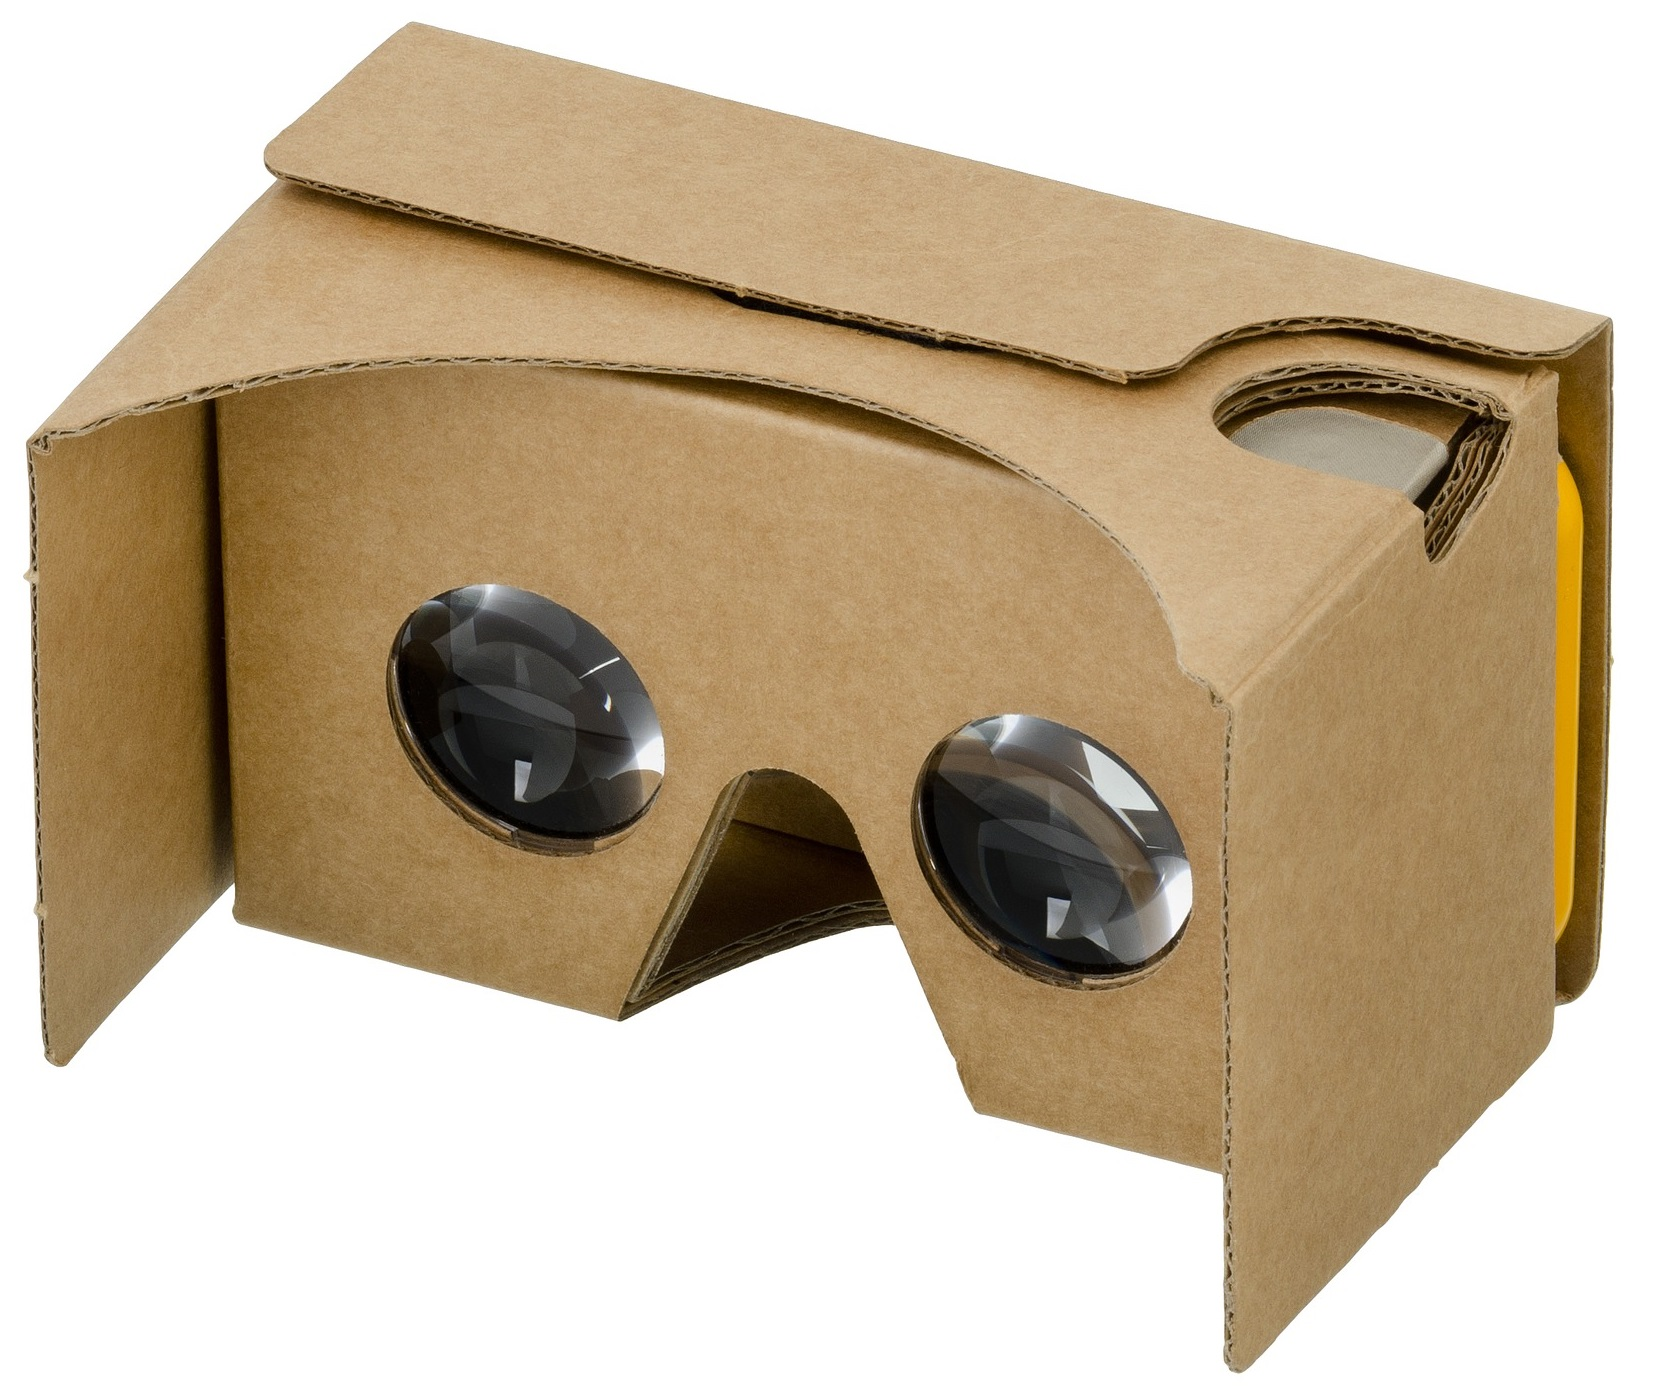
\includegraphics{img/google-cardboard.jpg}
          \caption{Google Cardboard für Smartphones}
          \label{fig:google-cardboard}
        \end{figure}
        Doch ist man durch das Fehlen der 3D-Eingaberäte bei dieser Lösung, je
        nach Anwendungsfall, etwas eingeschränkt. Je nach Smartphone kann auch eine geringe
        Bildschirmauflösung die in Kapitel \ref{Wahrnehmungsaspekte} genannten Aspekte
        beinträchtigen und einen Bruch der Illusionen hervorrufen.
        Projektionssysteme, die die simulierte Umgebung auf ganzen Leinwänden darstellen,
        haben den Vorteil, dass sich der Benutzer nicht unmittelbar vor dem Bildschirm
        befindet [\cite[134]{Dorner2013}]. Dadurch können keine einzelnen Pixel mit dem Auge 
        erfasst werden. Deshalb ist eins der kritischsten Kriterien bei einer VR-Brille 
        die Bildschirmauflösung [\cite[134]{Dorner2013}].
        Aktuelle Unternehmen die sich mit VR-Brillen beschäftigen und diese Technologie
        maßgeblich vorgeben, sind unter anderem  Facebook mit Oculus
        \footnote{Oculus | \url{https://www.oculus.com/?locale=de_DE} (18.10.2020)}, 
        HTC mit Vive \footnote{HTC VIVE | \url{https://www.vive.com/de/} (18.10.2020)},
        Playstation mit PlaystationVR
        \footnote{PlaystationVR | \url{https://www.playstation.com/de-de/explore/playstation-vr/} (18.10.2020)}
        und Valve Corporation mit der Valve Index
        \footnote{Valve Index | \url{https://www.valvesoftware.com/de/index/headset} (19.10.2020)}.
        Samsung beschäftigt sich ebenfalls mit Virtual
        Reality, jedoch bieten diese nur eine hochwertige Brille an ohne Rechenleistung.
        Für den vollständigen Funktionsumfang wird ein Samsung Smartphone vorausgesetzt
        \footnote{Samsung Gear VR | \url{https://www.samsung.com/de/wearables/gear-vr-r323/} (18.10.2020)}.
        Auch Nintendo hat mit ihrer Konsole Nintendo Switch den Weg zu Virtual Reality
        gefunden
        \footnote{Nintendo Labo VR-SET | \url{https://www.nintendo.de/Nintendo-Labo/Nintendo-Labo-1328637.html} (18.10.2020)}.
        Das VR-Set für die Nintendo Switch bietet sich gut für Kinder an, um erste 
        Erfahrungen mit Virtual Reality machen zu können.
        Aber auch Google ist in diesem Markt involviert, wie man an der zuvor erwähnten
        Google Cardboard (siehe. Abb. \ref{fig:google-cardboard}) sehen kann, bieten jedoch keine 
        VR-Brille mit integrierter Hardware.
      \subsubsection{Native und webbasierte Anwendungen}
        Viele VR-Brillen bedeuten auch viele SDKs die damit einhergehen. VR-Anwendungen
        können heutzutage mit Hilfe von vielen Programmen oder Frameworks entwickelt
        werden. Dabei bestehen die Möglichkeiten, nativ für eine Plattform zu entwickeln oder 
        auf webbasierte Anwendungen zurückzugreifen, die plattformunabhängig funktionieren. 
        Beide Wege bieten ihre Vor- und Nachteile, sind deshalb vom jeweiligen Anwendungsfall abhängig.
        Native Lösungen bieten in der Softwareentwicklung eine bessere 
        Performance, da diese Anwendungen mit Programmiersprachen entwickelt werden die
        effizient und maschinennah sind. Je nach Hersteller gibt es auch für das 
        Betriebssystem eigene Programmiersprachen, die dann auf das jeweilige Okösystem 
        optimiert sind.
        Webanwendungen, die in der Regel auf Basis von JavaScript laufen, werden nicht 
        kompiliert sondern interpretiert und der Quellcode wird zur Laufzeit vom Browser 
        gelesen und ausgeführt.
        Durch eine große und aktive Community hat sich JavaScript in den letzten Jahren 
        jedoch zu einer universellen Programmiersprache entwickelt und findet Anwendung in
        fast allen Gebieten der Softwareentwicklung.
        Die Entwicklung der letzten Jahre hat gezeigt, dass der Mensch weniger
        Zeit im Internet vor dem PC verbringt, sondern hauptsächlich mobil [\cite[1]{Ater2017}].
        Durch das Betrachten von Internetseiten auf einem mobilen Endgerät wurde der
        Ansatz mobile-first immer wichtiger [\cite[1]{Ater2017}]. Die Vorteile, die native
        Anwendungen mehrere Jahre mit sich brachten, waren, neben der besseren Leistung,
        erweiterte Grafikmöglichkeiten, Standortermittlung, Push-Benachrichtigungen,
        Offlineverfügbarkeit und Startbildschirm-Verknüpfungen [\cite[3]{Ater2017}]. Diese
        Funktionen waren damals notwendig für erfolgreiche Apps, da diese dem
        Benutzer eine bessere Nutzungserfahrung ermöglichten. Diese Funktionen sind nicht mehr
        nur nativen Anwendungen vorenthalten, sondern auch das Web als Plattform hat sich
        weiterentwickelt.
        Sogenannte Progressive Web Apps erlauben sich an native Funktionen der Plattform zu
        bedienen, bieten jedoch weiterhin die Flexibilität die das Web mit sich bringt
        [\cite[2]{Ater2017}].
        ServiceWorker machen es möglich, webbasierte Anwendungen 
        offlinefähig zu gestalten, Push-Benachrichtigungen können auch von Webseiten verschickt
        werden und über jeden modernen Browser lassen sich Desktop- oder 
        Startbildschirmverknüpfungen anlegen [\cite[5-6]{Ater2017}]. 
        Durch das Ausblenden der URL-Leiste des Browsers
        und Ausführen der webbasierten Anwendung im Vollbildmodus, fühlen sie sich wie
        native Anwendungen an [\cite[6]{Ater2017}]. Ist das Ziel einer Anwendung diese
        möglichst zugänglich zu machen, ist die Entwicklung einer webbasierten Lösung
        vorteilhaft, da man plattformunabhängig entwickeln kann und, sobald der
        Benutzer auf der Webseite ist, dieser direkt am Ziel ist. Es muss kein zusätzlicher
        Download oder eine zusätzliche Installation erfolgen und das Pflegen mehrerer
        Versionen in den verschiedenen App Stores entfällt. Der Benutzer kann unabhängig
        seiner Plattform und Gerät die Anwendung benutzen. Da der Benutzer an keine Plattform
        gebunden ist, gibt es dementsprechend auch ein vielfaches mehr an potenziellen
        Benutzern [\cite[3]{Ater2017}].
        Es ist zunehmend schwieriger geworden Benutzer zu einem Download einer App 
        zu motivieren [\cite[3]{Ater2017}].
        Die meisten Benutzer gehen bereits auf dem Weg zum jeweiligen Store und die darauffolgende
        Installation verloren [\cite[4]{Ater2017}]. APIs wie die Web Share und Web Share Target
        API sind nur ein Teil der zukünftigen Entwicklung, die immer mehr Funktionen ins
        Web bringen, welche zuvor nur für native Anwendungen zur Verfügung standen [\cite[245]{Ater2017}].
        Selbst Virtual Reality findet Anwendung im Browser durch die WebXR-Schnittstelle 
        (ehemals WebVR) [\cite[245]{Ater2017}]. In Kombination mit WebGL lassen sich komplexe,
        rechenintensive und überzeugende VR-Erfahrungen entwickeln [\cite[245]{Ater2017}].
        Die Schnittstelle WebXR ist kompatibel mit den gängigsten VR-Brillen und kann auch
        ihre jeweiligen 3D-Eingabegeräte lesen, wodurch der Entwickler Zugang zu allen Informationen
        bekommt, die auch eine native Desktop-Anwendung mitbringen würde [\cite[245]{Ater2017}].
        Im Punkt Leistung sind nach wie vor native Anwendungen einige Schritte voraus, doch
        gibt es jetzt schon bereits Lösungen, die an diesem Problem arbeiten. WebAssembly\footnote{Offizielle WebAssembly Webseite | \url{https://webassembly.org/} (02.11.2020)}
        ist eine niedere Programmiersprache, welche wenig Abstraktion zur Befehlssatzarchitektur
        des Computers bietet [\cite[185]{Haas2017Jun}]. Dadurch, dass WebAssembly zu ByteCode
        kompiliert wird, kann man nahezu native Leistung mit einer webbasierten Anwendung erreichen
        [\cite[186]{Haas2017Jun}]. Da WebAssembly über den Browser ausgeführt werden kann,
        bleibt weiterhin die Plattformunabhängigkeit geboten. Jedoch ist WebAssembly noch nicht
        so verbreitet wie JavaScript und bietet deshalb weniger Technologien und Möglichkeiten,
        damit VR-Anwendungen zu entwickeln. Zum aktuellen Zeitpunkt bietet die Unity Engine
        die Möglichkeit, unter anderem VR-Anwendungen mit Hilfe ihrer Engine zu entwickeln und
        diese für moderne Browser zu exportieren\footnote{WebAssembly in Unity | \url{https://blogs.unity3d.com/2018/08/15/webassembly-is-here/} (02.11.2020)}.
        Unreal Engine ist noch nicht auf WebAssembly umgestiegen, kompiliert den Code weiterhin
        zu JavaScript und hat die HTML5-Entwicklung sogar als Erweiterung ausgelagert, die durch
        die Community weiterentwickelt werden soll\footnote{Unreal Engine Dokumentation für HTML5 Development | \url{https://docs.unrealengine.com/en-US/Platforms/HTML5/index.html} (02.11.2020)}.
        Da es in der klassischen Softwareentwicklung nicht sinnvoll ist in Assemblersprache
        zu entwickeln, macht es genau so wenig Sinn selbstständig eine VR-Anwendung in 
        WebAssembly zu entwickeln. Deshalb wird eine höhere Programmiersprache benötigt die
        eine höhere Abstraktion bietet. So ist es am einfachsten Unity als Software zu nutzen,
        um VR-Anwendungen auf Basis von WebAssembly zu generieren.
        Nach wie vor ist die Entscheidung, ob man nativ oder für das Web entwickelt, abhängig
        vom Anwendungsfall. Für das Cranach Digital Archive bietet sich eine webbasierte Lösung
        an, da die Darstellung von Gemälden und Archivalien keine hochkomplexen Berechnungen
        benötigen. Das aktuelle Archiv ist über das Internet zu erreichen und lässt sich auf
        Desktop-PCs und mobile Endgeräte betrachten. Das Archiv ist bereits über die größte
        Plattform zu erreichen, dementsprechend sollte die VR-Lösung ebenfalls zugänglich
        über das Web sein. So können auch Kunstinteressierte, die sich keine hochwertige
        VR-Brille leisten möchten, die Gemälde und Archivalien mit ihrem Smartphone erkunden.
        Durch eine plattformunabhängige Lösung ist weniger Wartung notwendig und das
        Bereitstellen in die jeweiligen App Stores entfällt ebenfalls, was oft viel Zeit und
        Ressourcen in Anspruch nimmt [\cite[248]{Ater2017}]. Da webbasierte Anwendungen die
        wenigsten Ressourcen für eine hohe Zugänglichkeit benötigen, bietet sich dieser
        Entwicklungsansatz auch für das Forschungsprojekt an, da die vorhandenen Ressourcen
        gering sind.
        \subsubsection{Aktuelle Technologien}

    \subsection{Virtual Reality im musealen Kontext}
      Die Idee Kunst in einer virtuellen Realität darzustellen ist keine einzigartige Idee.
      Bereits andere Museen wagten sich daran und stellten Konzepte her, sammelten
      Erfahrungsberichte und entwickelten eigene Produkte. Es ist
      aber auch ein richtiger und verständlicher Schritt, dass Virtual Reality immer mehr
      im musealen Bereich Anwendung findet. Denn Museen versuchen Gefühle,
      Erfahrungen und Emotionen zu übermitteln und durch den Einsatz von Virtual Reality
      besteht die Möglichkeit den Besucher in Szenarien zu versetzen, die in der
      Vergangenheit geschehen sind. Der Besucher kann Fantasiewelten der Künstler
      wahrnehmen, um ein besseres Verständnis für ihre Kunst zu erlangen. Umfragen ergaben, 
      dass ein Interesse an neuartigen Technologien im Museum vorhanden ist [\cite[34]{Heidsiek2019}].
      Die Besucher erhoffen sich dadurch, dass die Museen unterhaltsamer, lehrreicher und
      zugänglicher werden [\cite[34]{Heidsiek2019}]. Gerade Virtual Reality lässt Museen
      und Informationen zugänglicher werden, denn die Besucher sind nicht mehr gezwungen 
      das Museum physisch zu besuchen. Der Anwendungsbereich ist vielfältig und die 
      Technologie zwar nicht neu, jedoch noch nicht ausgereizt.
      Doch birgen neue Technologien neben ihren Chancen aus Risiken, die berücksichtigt
      und disktutiert werden müssen. Deshalb wird in diesem Kapitel auf die
      Risiken und auch auf die Chancen eingegangen, die ein Museum bei einem Einsatz von
      Virtual Reality erwartet. Da das Cranach Digital Archive nicht das erste Museum ist, 
      welches Kunst digitalisiert, sollen bereits entwickelte Produkte analysiert und 
      werden deren Erkentnisse und Ideen dabei helfen, bereits begangene Fehler zu 
      vermeiden und geeignete Prototypen zu entwickeln.
      \subsubsection{Chancen und Risiken}
        Museen sind Stätten des Wissens. Ihre Aufgabe besteht darin, Menschen Wissen zu
        vermitteln, meist über vergangene Erfahrungen oder Geschehnisse. Durch die
        Digitalisierung und das Internet war es erstmals möglich, historische Gegenstände
        oder Gemälde mit der ganzen Welt zu teilen, unabhängig des Standorts des 
        Betrachters. Dementsprechend liegt der Mehrwert von digitalen Museen darin, eine
        erhöhte Vervielfältigung und Verbreitung von Wissen zu betreiben [\cite[17]{Huennekens2002}].
        Auch das Anwendunsgebiet Virtual Reality bietet nach dem Internet und der Digitalisierung
        eine neue Möglichkeit Informationen innovativ zu übermitteln [\cite[52]{Heidsiek2019}].
        So wird das Museum als Stätte des Wissens effizienter und ermöglicht mehr Menschen
        zu erreichen, als es vorher möglich war. Das Cranach Digital Archive geht hier mit
        gutem Beispiel voran und bietet eine riesige und strukturierte Datenbank an Wissen
        zu den Werken und Archivalien der Cranachs.
        Im Vergleich zu statischen Objekten, wie hängende Gemälde an Wänden, lassen sich 
        durch digitale Lösungen verschiedene und neue Darstellungen ermöglichen [\cite[17]{Huennekens2002}].
        Gerade Virtual Reality bietet hier eine sehr interessante Möglichkeit, völlig neue
        Perspektiven zu erschaffen, die niemals in der realen Welt erreicht werden können.
        Ein Vorteil in Virtual Reality liegt darin, dass die Gesetze von Raum und Zeit nicht
        in einer virtuellen Realität gelten [\cite[140]{Huennekens2002}]. So kann der Mensch
        seiner Begierde, alltägliche Erfahrungen zu überschreiten, nachkommen [\cite[140]{Huennekens2002}].
        Durch diese schier unendlichen Möglichkeiten kommt jedoch auch eine ethische 
        Verantwortung mit sich, wie man kunsthistorische Gegenstände präsentiert.
        Das Loslösen von Raum und Zeit kann sich negativ auf die historischen Inhalte auswirken
        [\cite[141]{Huennekens2002}]. Man spricht hier sogar von Entweihung der historischen
        Gegenstände [\cite[141]{Huennekens2002}]. Deshalb liegt es in der Verantwortung der
        Museen die historische Integrität eines Gegenstandes oder einer Erfahrung nicht
        zu verletzen [\cite[38]{Heidsiek2019}]. Das kann aber vermieden werden, in dem 
        kenntlich gemacht wird, was original ist und was selbstständig hinzugefügt
        wurde [\cite[38]{Heidsiek2019}]. Sobald virtuelle Realitäten erfundene Aspekte 
        beinhalten, und diese nicht als solche gekennzeichnet wurden, handelt es sich nicht
        mehr um eine historische Überlieferung, sondern um persönliche und subjektive 
        Wahrnehmungen [\cite[38]{Heidsiek2019}]. Durch fotorealistische Darstellungen
        von unwahren Ereignissen oder Objekte können verstärkt dazu führen, dass der
        Benutzer überzeugt von der fälschlichen Tatsache wird [\cite[39]{Heidsiek2019}].
        So hat jedes Museum, dass Virtual Reality als Möglichkeit zur Betrachtung 
        kunstrelevanter Objekte anbieten möchte, die ethische Verantwortung, 
        dem Benutzer zu jedem Zeitpunkt kenntlich zu machen,
        was eine historische Übermittlung und was virtuelle Realität ist.
        Doch besteht durch Virtual Reality die Gefahr, dass Museen auf lange Sicht 
        betrachtet obsolet werden und alles über eine VR-Brille erforscht werden kann
        [\cite[142-143]{Huennekens2002}]? Besucher die Virtual Reality in Museen genutzt
        haben, betrachten diese Technologie jedoch als Ergänzung zum Museum und nicht als
        einen vollständigen Ersatz, da der Hauptgrund eines Museumsbesuch die 
        Originalobjekte sind [\cite[79]{Heidsiek2019}]. Originale Ausstellungsstücke
        haben nach wie vor einen nicht reproduzierbaren Charakter, welcher sich in einer
        virtuellen Realität darstellen lässt [\cite[93]{Heidsiek2019}]. Im Gegenteil,
        Darstellungen von Originalobjekten als Kopie in einer virtuellen Welt schwächt
        sogar die Authentizität dieser [\cite[93]{Heidsiek2019}]. 
        Besucher, die vorher eine Online-Ausstellung eines Museums gesehen haben,
        entschieden sich sogar aufgrund dessen für das Besuchen des Museums in der 
        realen Welt [\cite[777-778]{Katz2015}]. So kann eine VR-Erfahrung, die über
        das Web zu erreichen ist, nicht als Ersatz für das Museum gesehen werden,
        sondern auch als innovatives und modernes Marketingwerkzeug.
        Dementsprechend ist nach aktuellem
        Stand nicht davon auszugehen, dass die Technologie Virtual Reality das Museum in
        naher oder mittlerer Zukunft obsolet macht.
        Die Museumslandschaft sieht in Virtual Reality die Chancen, neue und andere
        Geschichten zu vermitteln, langfristig für Besucher attraktiv zu bleiben und
        auch eine neue Zielgruppe zu erreichen [\cite[34-35]{Heidsiek2019}].
        Da Emotionen Teil eines Museumsbesuch sind, lassen sich durch den Einsatz
        von Virtual Reality neue und intensivere Emotionen hervorrufen. Empfundene 
        Emotionen bei einem Lernprozess tragen nachweislich zu einem erhöhten Lernerfolg
        bei [\cite[29]{Heidsiek2019}]. So konnte nachgewiesen werden, dass VR-Erfahrungen
        bei musealen Ausstellungen zu erhöhtem Interesse, erhöhter Zufriedenheit und 
        Vergnügen geführt haben [\cite[69-72]{Heidsiek2019}]. Dadurch können schwer
        verständliche Themen leichter übermittelt werden und der Informationsaustausch
        zwischen Museum und Mensch optimiert werden. Das deckt sich auch mit der Chance,
        langfristig für Besucher attraktiv zu bleiben und eine neue Zielgruppe anzusprechen,
        die vorher nichts mit Museen anfangen konnten.
        Aber auch die aktuelle Zielgruppe eines Museums kann etwas mit Virtual Reality
        anfangen, unabhängig des Alters [\cite[75]{Heidsiek2019}]. Dadurch wird keine 
        bestimmte Zielgruppe ausgeschlossen.
      \subsubsection{Optimierung des Lernprozesses}
        Wie bereits im vorherigen Unterkapitel erwähnt, tragen Emotionen nachweislich zum
        Lernerfolg bei. Um diese Emotionen bei Besuchern zu aktivieren und entsprechende
        Gefühle hervorzurufen, bietet es sich an, Lebensräume der darzustellenden Personen
        oder Objekte in der virtuellen Welt nachzustellen [\cite[35-36]{Heidsiek2019}].
        Anhand dessen kann sich der Benutzer noch besser in die Situation hineinbegeben
        und komplexe Gefühle und Emotionen besser wahrnehmen. Storytelling stellt hierbei
        eine mögliche Methode dar [\cite[35-39]{Heidsiek2019}].
        Bei VR-Erfahrungen im Museum lassen sich zwei Emotionen beobachten: 
        Die erfahrungsbezogene und inhaltsbezogene Emotion [\cite[69]{Heidsiek2019}]. 
        Erstere beschreibt die
        empfundene Emotion die während der gesamten Nutzungserfahrung entstanden ist und
        letztere die Emotion, die empfunden wird, während sich mit einem genauen
        Ausstellungsstück beschäftigt wird. Virtual Reality ruft vermehrt die 
        erfahrungsbezogenen Emotionen hervor [\cite[69]{Heidsiek2019}], was im Hinblick auf
        die Technologie jedoch logischt erscheint. Denn durch Virtual Reality liegt der
        Fokus nicht nur auf genau einem einzigen Objekt, sondern meist auf eine ganze
        Szene und die Erfahrung innerhalb dieser. Die erfahrungsbezogenen Emotionen 
        sind diejenigen, die einen besseren
        Lerneffekt mit sich bringen und Museen werden dadurch als unterhaltsamer und
        aufregender bezeichnet [\cite[69]{Heidsiek2019}]. Traditionelle Museen rufen 
        hauptsächlich inhaltsbezogene Emotionen hervor [\cite[69]{Heidsiek2019}], da der
        Fokus bei Ausstellungen oft auf einzelnen Ausstellungsstücke liegt.
        Immersive Umgebungen, die Virtual Reality in hoher Form bieten können, tragen ebenfalls
        zu einem optimierten Lernprozess bei, da der Lernende den Inhalt selbstständig steuern
        und manipulieren kann [\cite[777]{Katz2015}]. Ebenso kann der Lernende
        die Lerngeschwindigkeit selbstständig bestimmen [\cite[777]{Katz2015}],
        was die Konzentration erhöht. Nichtsdestotrotz muss berücksichtigt werden,
        dass nicht jeder Anwender sofort perfekt mit der virtuellen Umgebung agieren
        kann. So kann durch zu komplizierte Interaktionen und Darstellungen
        eher eine negative Erfahrung hervorbringen, was dem Lernprozess eher
        schadet [\cite[777]{Katz2015}]. An dieser Stelle kann man sich an die
        Studie des Deutschen Auswandererhauses richten, welche eine einfache
        Bedienung durch blickgesteuerte Interaktion gewährleisteten [\cite[38]{Heidsiek2019}].
        Dadurch müssen die Benutzer nur noch eine Brille aufsetzen und können
        sofort innerhalb der Anwendung navigieren, da keine Tasten der Eingabegeräte
        auswendig gelernt werden müssen.
        Auch das Gefühl der Präsenz, welches bereits in Kapitel \ref{Wahrnehmungsaspekte}
        behandelt wurde, trägt dazu bei, wie gut der Lernende Informationen aufnimmt
        [\cite[777]{Katz2015}].
      \subsubsection{Aktuelle Lösungen und Umsetzung}
        Da es viele Technologien und Hardware für die Umsetzung von VR-Ausstellungen 
        gibt, lassen sich auf viele verschiedene Wege solche VR-Erfahrungen entwickeln.
        Das Deutsche Auswandererhaus beispielsweise entschied sich für das Samsung Odyssey
        Virtual Reality Headset, welches ohne Controller funktionieren sollte und intuitiv
        bedienbar ist [\cite[35]{Heidsiek2019}]. Sie entwickelten eine VR-Erfahrung, die
        mittels Storytelling vermittelt wurde [\cite[35-39]{Heidsiek2019}]. Dabei
        konnte man zwei VR-Erfahrungen erleben. Eine bestand aus einer auditiven und
        blickgesteuerten Interaktion und die andere aus einem 360-Grad-Video [\cite[38]{Heidsiek2019}].
        Aufgrund der positiven Studienergebnisse und Bewertungen der Probanten, scheint
        die Entwicklung einer VR-Erfahrung mit blickgesteuerter Interaktion sinnvoll, da
        keine Einarbeit in die Eingabegeräte der VR-Brille notwendig ist. Dadurch erhält
        die Anwendung eine intuitive Steuerung. Auch das vermitteln einer Geschichte 
        innerhalb der VR-Erfahrung fördert das Interesse der Benutzer [\cite[35-39]{Heidsiek2019}].
        Google bietet ebenfalls eine simple Anwendung, die über ein Google Daydream
        kompatibles Smartphone ausgeführt werden kann\footnote{Google Arts \& Culture VR | \url{https://play.google.com/store/apps/details?id=com.google.vr.museums&hl=de} (04.11.2020)}.
        Hierbei lassen sich Gemälde betrachten und nah an diese heranzoomen.
        Besondere Funktionen oder ein Storytelling weist diese App nicht auf. Sie immitiert
        letztlich ein Museumsbesuch in einer virtuellen Welt nach.
  \section{Prototyping}
    Das Prototyping ist eine Methode in der Softwareentwicklung, um schnell an
    Ergebnisse zu gelangen. Anhand eines Prototypen kann schnell erkannt werden,
    ob eine Idee technisch umsetzbar ist und was noch benötigt wird, um das Produkt
    zu verbessern. Je nach Fortschritt des Prototypen können auch schon Nutzererfahrungen
    und Feedback gesammelt werden.
    Diese Methode wird in diesem Forschungsprojekt angewandt, um mehrere Ergebnisse
    zu erzielen und zu erörtern, welche technischen Möglichkeiten heutzutage existieren.
    [\cite{Bertsche2007}]
    \subsection{Auswahl der Technologie}
    
    \subsection{Umsetzung der Softwareentwicklung}
  \section{Ergebnisse}
    \begin{itemize}
      \item Hier verwendet man beschriebene Methoden an
      \item Beschreiben, wie Untersuchung verlaufen ist
      \item Ergebnisse analysieren
    \end{itemize}
  \section{Diskussion und Fazit}
    \begin{itemize}
      \item Folgen und Ursache der Ergebnisse beschreiben
      \item Limitationen und Vorschläge für zukünftige Projekte darlegen
    \end{itemize}
    -
    \begin{itemize}
      \item Auf wichtigste Ergebnisse eingehen
      \item Geht auf Einleitung ein, da auf Forschungsfrage eingeht
      \item Füge keine neuen Informationen und Interpretationen
      \item Füge keine Beispiele und Zitate ein, bleibe bei den Fakten
      \item Dein Ergebnis ist immer wertvoll
      \item Ergebnisse deiner Forschung werden im Präsens geschrieben
    \end{itemize}
  \section{Anhang}
    \subsection{Abbildungen}
    \subsection{Literaturverzeichnis}
      \printbibliography
    \subsection{Abbildungsverzeichnis}
    \subsection{Eidesstattliche Erklärung} 
\end{document}